\section{Einführung}
In diesem Versuch wird die optische Abbildung anhand einer digitalen Kamera untersucht.
Bei einer digitalen Kamera werden Gegenstände über Linsen auf einen Bildsensor (CMOS) abgebildet. Da die Abbildung am Rand der Linse deutlich schlechter wird, begrenzt man durch eine Blende mit Durchmesser $D$ den Lichtverlauf auf die Mitte.

\subsection{Auflösung}
Durch Beugungseffekte an der Blende werden auch Puntquellen nicht als Punkte, sondern als "Beugungsscheibchen" abebildet. Je größer der Durchmesser dieser Scheibchen, desto unschärfer wird das Bild. Das \emph{Rayleigh}-Kriterium besagt, dass zwei Punktquellen gerade noch unterscheidbar sind, wenn das Maximum der ersten mit dem 1. Minimum der zweiten Abbildung übereinanderliegt. Ein Beugungsscheibchen bei einer Wellenlänge $\lambda$ bei Linse mit Brennweite $f$ und Apertur $D$ hat den Durchmesser\footcite{anleitung-ss2015}
\begin{equation}
	d=2,4392...\cdot\lambda\cdot\frac{f}{D}
\label{eq:rayleigh}
\end{equation}
Der Wert 
\begin{equation}
	k=\frac{f}{D}
\label{eq:blendenzahl}
\end{equation}
heißt Blendenzahl.

\subsection{Schärfentiefe}
Da die digitale Kamera über eine oder mehrere Linsen im Objektiv abbildet, gibt es analog zur Brennweite einer Linse bei der Kamera eine Fokusentfernung $g$. Gegenstände, die den Abstand $g$ zur Kamera haben (sich in der Fokusebene befinden), werden mit maximaler Schärfe abgebildet. Ist ein Gegenstand näher oder weiter von der Kamera entfernt, verschlechtert sich die Schärfe. Der Nah- bzw. Fernpunkt ist der Punkt am nähesten bzw. am entferntesten zur Kamera, an dem ein Gegenstand noch ausreichend scharf abgebildet werden kann. Ausreichend scharf bedeutet, dass der Durchmesser der Zerstreuungskreise $Z$ einen bestimmten Wert nicht überschreitet (typischerweise $1/1500$ der Bilddiagonalen\footcite{anleitung-ss2015}). Ab einer bestimmten Fokusentfernung, der hyperfokalen Entfernung $d_h$, rückt der Fernpunkt ins Unendliche, d.h. scharfe Abbildung ist für beliebig weit hinter dem Nahpunkt liegende Gegenstände möglich.
\\
Die hyperfokale Entfernung beträgt

\begin{equation}
	d_h=\frac{f^2}{kZ}+f=f\cdot \left(\frac{D}{Z}+1\right)
\label{eq:hyperfok}
\end{equation}

Der Nahpunkt liegt bei 

\begin{equation}
	d_n=\frac{g(d_h-f)}{(d_h-f)+(g-f)}=\frac{g}{\frac{g-f}{d_h-f}+1}
\label{eq:nahpunkt}
\end{equation}

und der Fernpunkt bei

\begin{equation}
	d_f=\begin{cases}
		\frac{g(d_h-f)}{(d_h-f)+(f-g)}=\frac{g}{\frac{f-g}{d_h-f}} & g<d_h \\
		\infty & g \geq d_h
		\end{cases}
\label{eq:fernpunkt}
\end{equation}

\subsection{MTF}
Um die Auflösung quantitativ anzugeben, wird die Modulationsübertragunsfunktion MTF genutzt. Sei $\nu$ die Linienfrequenz eines Musters, d.h. die Dichte der Linien (Einheit z.B. Linienpaare pro Bildhöhe $lp/ph$). Ist $V_{\text{max}}$ der Grauwert des schwarzesten und $V_{\text{min}}$ der Grauwert des weißesten Pixels im Bild, so berechnet sich der Kontrast durch
\begin{equation}
	C(\nu)=\frac{V_{\text{max}}-V_{\text{min}}}{V_{\text{max}}+V_{\text{min}}}\qquad .
\label{eq:kontrast}
\end{equation}
Für $C(0)$ werden die Grauwerte bei einem vollständig schwarzen bzw. weißen Muster genommen. Dann ist die MTF das Kontrastverhältnis
\begin{equation}
	MTF(\nu)=C(\nu)/C(0)\qquad .
\label{eq:mtf}
\end{equation}
Eine Methode zur Messung der Linienpaaren ist der Siemensstern. In der Mitte des Sterns ist die Linienfrequenz so groß, dass nur noch eine graue Fläche abgebildet wird. Aus dem Durchmesser $d$ dieser Fläche und der Anzahl der Sektoren $n$ berechnet man die Auflösung in Linienpaaren
\begin{equation}
	l=\frac{n}{\pi d}\qquad .
\label{eq:siemens}
\end{equation}
\begin{figure}[h]
  \centering
  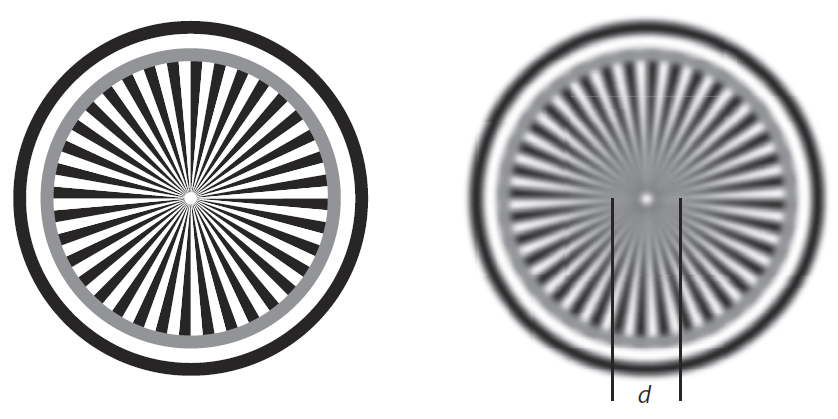
\includegraphics[width=.5\textwidth]{res/siemens}
  \caption{Siemensstern zur Bestimmung der Auflösung}
  \label{fig:siemens}
\end{figure}
Eine weitere Methode ist die der "schrägen Kante". Dabei wird ein Foto einer schrägen schwarzen Kante auf weißem Hintergrund aufgenommen. Aus dem Verlauf der Grauwerte an der Kante wird durch Differentiation und anschließende Fouriertransformation die MTF bestimmt.

\section{Versuche}
Die Kamera ist eine Nikon D3200 mit einem CMOS-Sensor der Größe $23.2 \times 15.4$ mm und einer Pixelzahl von $6016 \times 4000$ Pixel.
\subsection{Schärfentiefe}
Ein schräger Testchart mit aufgedrucktem Millimetermaß wird in ca. \SI{1}{m} Entfernung bei verschiedenen Blendenzahen abfotografiert. Die Schärfentiefe wird am PC-Monitor subjektiv beurteil und aus der 